% !TeX program = lualatex
\documentclass[12pt, a4paper]{article}
\usepackage{fullpage}
\usepackage{subfiles}
\usepackage{fontspec}
\usepackage{libertine}
\usepackage{xcolor}
\usepackage{GotIn}
\usepackage{geometry}
\usepackage{multicol}
\usepackage{multicolrule}
\usepackage{graphicx}
\usepackage{enumitem}
\usepackage[autocompile]{gregoriotex}
\usepackage[latin,french]{babel}


\geometry{top=2cm, bottom=2cm}
% \pagestyle{empty}

\definecolor{red}{HTML}{C70039}
% \input GoudyIn.fd
% \newcommand*\initfamily{\usefont{U}{GoudyIn}{xl}{n}}

\input Acorn.fd
\newcommand*\initfamily{\usefont{U}{Acorn}{xl}{n}}
% cette ligne ajoute de l'espace entre les portées
% \grechangedim{baselineskip}{60pt}{scalable}

\begin{document}
  \gresetlinecolor{gregoriocolor}

  \begin{titlepage}\centering
    \vspace*{\fill}\
    \huge Secondes Vêpres\\
    \smallskip
    \begin{Large}
      \textit{
        Fête du Sacré-Cœur\\
      }
    \end{Large}
    \medskip
    \large et\\
    \medskip
    \LARGE Salut du Saint-Sacrement\\
    \bigskip
    % \begin{figure}[h!]
    %   \centering
    %   
\includegraphics[width=7cm]{../ordinaires/logo.png}
    % \end{figure}
    \vspace*{\fill}
    \begin{figure}[h!]
      \centering
      
\includegraphics[width=7cm]{../ordinaires/logo.png}
    \end{figure}
    \centering \normalsize Paroisse Saint Roch\\
    \bigskip
    \begin{Large}
      \centering Ne pas emporter
    \end{Large}
  \end{titlepage}

  \newpage
  \vspace*{\fill}
    \begin{center}
      \normalsize\textit{
        Livret latin-français
      }
    \end{center}
  \newpage

  \begin{center}
    \textcolor{red}{\large{Ouverture.}}
  \end{center}

  % greillumination: remplace la première lettre, ici par une font ornementale
  \greillumination{\initfamily\fontsize{11mm}{11mm}\selectfont D}
  \gregorioscore{../ordinaires/vepres-deus_in_adjutorium}

  \begin{center}
    \small{
    \emph{
      Dieu, venez à mon aide ; Seigneur, hatez-vous de me secourir.\\
      Gloire au Père, au Fils et au Saint Esprit, comme il était au commencement, maintenant et toujour et dans les siècles des siècles. Allelúia\\
    }
  }
  \end{center}

  \newpage
  \normalsize

  % ===== DEBUT Antienne =========
  \gresetinitiallines{1}
  \greillumination{\initfamily\fontsize{11mm}{11mm}\selectfont U}
  \gregorioscore{antiennes/an--unus_militum--solesmes_1961}
  \begin{center}
    \footnotesize{
      \textit{Un des soldats lui ouvrit le côté avec une lance, et aussitôt il en sortit du sang et de l’eau. }
    }
  \end{center}
  % ===== FIN Antienne ===========

  % ===== DEBUT psaume ===========
  % gresetinitiallines : avec le parametre à 0, supprime l'ornement
  \begin{center}
    \large{Psaume 109.}\\
  \end{center}

  \gresetinitiallines{0}
  \gregorioscore{psaumes/psaume109-If}

  \begin{enumerate}[label=\textcolor{red}{\arabic*}]
    \setcounter{enumi}{1}
    \item Donec ponam ini\textbf{mí}cos \textbf{tu}os,\textcolor{red}{~*} scabéllum pe\textit{dum} \textit{tu}\textbf{ó}rum.

    \item Virgam virtútis tuæ emíttet Dómi\textbf{nus} ex \textbf{Si}on:\textcolor{red}{~*} domináre in médio inimicó\textit{rum} \textit{tu}\textbf{ó}rum.

    \item Tecum princípium in die virtútis tuæ in splendóri\textbf{bus} sanc\textbf{tó}rum:\textcolor{red}{~*} ex útero ante lucíferum \textit{gé}\textit{nu}\textbf{i} te.

    \item Jurávit Dóminus, et non pœni\textbf{té}bit \textbf{e}um:\textcolor{red}{~*} Tu es sacérdos in ætérnum secúndum órdi\textit{nem} \textit{Mel}\textbf{chí}sedech.

    \item Dóminus a \textbf{dex}tris \textbf{tu}is,\textcolor{red}{~*} confrégit in die iræ \textit{su}\textit{æ} \textbf{re}ges.

    \item Judicábit in natiónibus, im\textbf{plé}bit ru\textbf{í}nas:\textcolor{red}{~*} conquassábit cápita in ter\textit{ra} \textit{mul}\textbf{tó}rum.

    \item De torrénte in \textbf{vi}a \textbf{bi}bet:\textcolor{red}{~*} proptérea exal\textit{tá}\textit{bit} \textbf{ca}put.

    \item Glória \textbf{Pa}tri, et \textbf{Fí}lio,\textcolor{red}{~*} et Spirí\textit{tu}\textit{i} \textbf{Sanc}to.

    \item Sicut erat in princípio, et \textbf{nunc}, et \textbf{sem}per,\textcolor{red}{~*} et in sǽcula sæcu\textit{ló}\textit{rum}. \textbf{A}men.
  \end{enumerate}
  %  Répetition de l'Antienne
  \grecommentary{\textit{Reprise de l'Antienne.}}
  \gabcsnippet{(c4) U(d)nus(e_[uh:l]f) mí(g)li(g)tum(g.) (,) lán(gh)ce(g)a(g') la(g)tus(g') e(e)jus(gh) a(fe)pé(d)ru(cd)it(d.) (;) et(f) con(f)tí(fg)nu(f)o(c'_[oh:h]) (,) ex(d)í(dc)vit(f) san(e_[uh:l]f)guis(g) et(fe) a(d.)qua.(d.) (::)}

  \newpage
  \vspace*{\fill}\
  \begin{normalsize}
    \begin{center}
      \par \textit{Un des soldats lui ouvrit le côté avec une lance, et aussitôt il en sortit du sang et de l’eau. }
      \medskip
      \begin{enumerate}[label=\textcolor{red}{\emph{\arabic*}}]
        \item \textit{Le Seigneur a dit à mon Seigneur : Asseyez-toi à ma droite, }
        \item \textit{Jusqu'à ce que je mette tes ennemis pour le marchepied de tes pieds.}
        \item \textit{L'Éternel enverra de Sion la verge de ta force: Domine au milieu de tes ennemis!}
        \item \textit{Ton peuple sera un peuple de franche volonté, au jour de ta puissance, en sainte magnificence. Du sein de l'aurore te viendra la rosée de ta jeunesse.}
        \item \textit{L'Éternel a juré, et il ne se repentira point: Tu es sacrificateur pour toujours, selon l'ordre de Melchisédec.}
        \item \textit{Le Seigneur, à ta droite, brisera les rois au jour de sa colère.}
        \item \textit{Il jugera parmi les nations, il remplira tout de corps morts, il brisera le chef d'un grand pays.}
        \item \textit{Il boira du torrent dans le chemin, c'est pourquoi il lèvera haut la tête.}
        \item \textit{Gloire au Père, au Fils, et au Saint Esprit, }
        \item \textit{Comme il était au commencement, maintenant et toujours, et dans les siècles des siècles. Amen. }
      \end{enumerate}
    \end{center}
  \end{normalsize}
  \vspace*{\fill}\
  \newpage

  % ===== DEBUT Antienne =========
  \gresetinitiallines{1}
  \greillumination{\initfamily\fontsize{11mm}{11mm}\selectfont S}
  \gregorioscore{antiennes/an--stans_jesus--solesmes_1961}
  \begin{center}
    \footnotesize{
      \textit{Jésus se tenait debout et criait, en disant : Si quelqu’un a soif, qu’il vienne à Moi, et qu’il boive.}
    }
  \end{center}
  % ===== FIN Antienne ===========

  % ===== DEBUT psaume ===========
  % gresetinitiallines : avec le parametre à 0, supprime l'ornement
  \begin{center}
    \large{Psaume 110.}\\
  \end{center}

  \gresetinitiallines{0}
  \gregorioscore{psaumes/psaume110-VIIc}

  \begin{enumerate}[label=\textcolor{red}{\arabic*}]
    \setcounter{enumi}{1}
    \item Magna \textbf{ó}pera \textbf{Dó}mini:\textcolor{red}{~*} exquisíta in omnes volun\textbf{tá}tes \textbf{e}jus.

    \item Conféssio et magnificéntia \textbf{o}pus \textbf{e}jus:\textcolor{red}{~*} et justítia ejus manet in \textbf{sǽ}culum \textbf{sǽ}culi.

    \item Memóriam fecit mirabílium suórum,\textcolor{red}{~†}  miséricors et mise\textbf{rá}tor \textbf{Dó}minus:\textcolor{red}{~*} escam dedit ti\textbf{mén}ti\textbf{bus} se.

    \item Memor erit in sǽculum testa\textbf{mén}ti \textbf{su}i:\textcolor{red}{~*} virtútem óperum suórum annuntiábit \textbf{pó}pulo \textbf{su}o:

    \item Ut det illis heredi\textbf{tá}tem \textbf{gén}tium:\textcolor{red}{~*} ópera mánuum ejus véritas, \textbf{et} ju\textbf{dí}cium.

    \item Fidélia ómnia mandáta ejus:\textcolor{red}{~†}  confirmáta in \textbf{sǽ}culum \textbf{sǽ}culi,\textcolor{red}{~*} facta in veritáte et \textbf{æ}qui\textbf{tá}te.

    \item Redemptiónem misit \textbf{pó}pulo \textbf{su}o:\textcolor{red}{~*} mandávit in ætérnum testa\textbf{mén}tum \textbf{su}um.

    \item Sanctum, et terríbile \textbf{no}men \textbf{e}jus:\textcolor{red}{~*} inítium sapiéntiæ \textbf{ti}mor \textbf{Dó}mini.

    \item Intelléctus bonus ómnibus faci\textbf{én}tibus \textbf{e}um:\textcolor{red}{~*} laudátio ejus manet in \textbf{sǽ}culum \textbf{sǽ}culi.

    \item Glória \textbf{Pa}tri, et \textbf{Fí}lio,\textcolor{red}{~*} et Spi\textbf{rí}tui \textbf{Sanc}to.

    \item Sicut erat in princípio, et \textbf{nunc}, et \textbf{sem}per,\textcolor{red}{~*} et in sǽcula sæcu\textbf{ló}rum. \textbf{A}men.
  \end{enumerate}
  %  Répetition de l'Antienne
  \grecommentary{\textit{Reprise de l'Antienne.}}
  \gabcsnippet{(c3) Stans(ig) Je(ij)sus(ijji.) (,) cla(g_[uh:l]h)má(i)bat(f') di(e)cens :(e.) (;) Si(e) quis(g) si(e_[uh:l]f)tit,(f') (,) vé(g)ni(hi)at(i) ad(hg/hf~) me(gh'i) et(h_) bi(e.)bat.(e.) (::)}

  \newpage
  \vspace*{\fill}\
  \begin{normalsize}
    \begin{center}
      \par \textit{Jésus se tenait debout et criait, en disant : Si quelqu’un a soif, qu’il vienne à Moi, et qu’il boive.}
      \medskip
      \begin{enumerate}[label=\textcolor{red}{\emph{\arabic*}}]
        \item \textit{De tout cœur je rendrai grâce au Seigneur dans l'assemblée, parmi les justes.}
        \item \textit{Grandes sont les œuvres du Seigneur ; tous ceux qui les aiment s'en instruisent.}
        \item \textit{Noblesse et beauté dans ses actions : à jamais se maintiendra sa justice.}
        \item \textit{De ses merveilles il a laissé un mémorial ; le Seigneur est tendresse et pitié, il a donné des vivres à ses fidèles,}
        \item \textit{Gardant toujours mémoire de son
        alliance, il a montré sa force à son peuple.}
        \item \textit{Lui donnant le domaine des nations. Justesse et sûreté les œuvres de ses mains.}
        \item \textit{Sécurité, toutes ses lois, établies pour toujours et à jamais, accomplies avec droiture et sûreté ! }
        \item \textit{Il apporte la délivrance à son peuple ; son alliance est promulguée pour toujours.}
        \item \textit{Saint, redoutable est son nom, la sagesse commence avec la crainte du Seigneur.}
        \item \textit{Qui accomplit sa volonté en est éclairé. A jamais se maintiendra sa louange.}
        \item \textit{Gloire au Père, au Fils, et au Saint Esprit, }
        \item \textit{Comme il était au commencement, maintenant et toujours, et dans les siècles des siècles. Amen. }
      \end{enumerate}
    \end{center}
  \end{normalsize}
  \vspace*{\fill}\
  \newpage

  % ===== DEBUT Antienne =========
  \gresetinitiallines{1}
  \greillumination{\initfamily\fontsize{11mm}{11mm}\selectfont I}
  \gregorioscore{antiennes/an--in_caritate_perpetua--solesmes}
  \begin{center}
    \footnotesize{
      \textit{D’un amour éternel Dieu nous a aimé, c’est pourquoi, élevé de terre, il nous a attiré à son Cœur, par compassion. }
    }
  \end{center}
  % ===== FIN Antienne ===========

  % ===== DEBUT psaume ===========
  % gresetinitiallines : avec le parametre à 0, supprime l'ornement
  \begin{center}
    \large{Psaume 115.}\\
  \end{center}

  \gresetinitiallines{0}
  \gregorioscore{psaumes/psaume115-IIIa2}

  \begin{enumerate}[label=\textcolor{red}{\arabic*}]
    \setcounter{enumi}{1}
    \item Ego dixi in ex\textbf{cés}su \textbf{me}o:\textcolor{red}{~*} Omnis \textit{ho}\textit{mo} \textbf{men}dax.

    \item Quid re\textbf{trí}buam \textbf{Dó}\textbf{mi}no,\textcolor{red}{~*} pro ómnibus, quæ retrí\textit{bu}\textit{it} \textbf{mi}hi?

    \item Cálicem salu\textbf{tá}ris ac\textbf{cí}\textbf{pi}am:\textcolor{red}{~*} et nomen Dómini \textit{in}\textit{vo}\textbf{cá}bo.

    \item Vota mea Dómino reddam coram omni \textbf{pó}pulo \textbf{e}jus:\textcolor{red}{~*} pretiósa in conspéctu Dómini mors sanc\textit{tó}\textit{rum} \textbf{e}jus:

    \item O Dómine, quia ego \textbf{ser}vus \textbf{tu}us:\textcolor{red}{~*} ego servus tuus, et fílius an\textit{cíl}\textit{læ} \textbf{tu}æ.

    \item Dirupísti víncula mea:\textcolor{red}{~†}  tibi sacrificábo \textbf{hós}tiam \textbf{lau}dis,\textcolor{red}{~*} et nomen Dómini \textit{in}\textit{vo}\textbf{cá}bo.

    \item Vota mea Dómino reddam in conspéctu omnis \textbf{pó}puli \textbf{e}jus:\textcolor{red}{~*} in átriis domus Dómini, in médio tu\textit{i}, \textit{Je}\textbf{rú}salem.

    \item Glória \textbf{Pa}tri, et \textbf{Fí}\textbf{li}o,\textcolor{red}{~*} et Spirí\textit{tu}\textit{i} \textbf{Sanc}to.

    \item Sicut erat in princípio, et \textbf{nunc}, et \textbf{sem}per,\textcolor{red}{~*} et in sǽcula sæcu\textit{ló}\textit{rum}. \textbf{A}men.
  \end{enumerate}
  %  Répetition de l'Antienne
  \grecommentary{\textit{Reprise de l'Antienne.}}
  \gabcsnippet{(c4) In(e) ca(f)ri(ed)tá(g)te(h') per(g)pé(hj)tu(j)a(i.) (,) di(i_j)lé(k)xit(ji) nos(hi) De(g)us,(g.) (;) í(g)de(hi)o(i) ex(i)al(i)tá(j)tus(hg) a(h) ter(hi)ra,(i.) (,) at(g)trá(e)xit(fe~) nos(d.) (;) ad(dh) Cor(gf) su(g)um(ghg) mí(e)se(de)rans.(e.) (::)}

  \newpage
  \vspace*{\fill}\
  \begin{normalsize}
    \begin{center}
      \par \textit{D’un amour éternel Dieu nous a aimé, c’est pourquoi, élevé de terre, il nous a attiré à son Cœur, par compassion. }
      \medskip
      \begin{enumerate}[label=\textcolor{red}{\emph{\arabic*}}]
        \item \textit{J’ai cru, c’est pourquoi j’ai parlé : je suis dans une humiliation extrême.}
        \item \textit{J’ai dit dans l’excès de ma douleur : Tout homme est menteur.}
        \item \textit{Que rendrai-je au Seigneur, pour tous les biens qu’il m’a faits ?}
        \item \textit{Je prendrai le Calice du salut, et j’invoquerai le nom du Seigneur. }
        \item \textit{Je rendrai mes vœux au Seigneur en présence de tout son peuple : précieuse est la mort de ses Saints aux yeux du Seigneur.}
        \item \textit{O Seigneur, parce que je suis ton serviteur, et le fils de ta servante. }
        \item \textit{Tu as brisé mes liens : je te sacrifierai un sacrifice de louange, et j’invoquerai le nom du Seigneur.}
        \item \textit{Je rendrai mes vœux au Seigneur devant tout son peuple ; dans le vestibule de la maison du Seigneur, au milieu de toi, ô Jérusalem. }
        \item \textit{Gloire au Père, au Fils, et au Saint Esprit, }
        \item \textit{Comme il était au commencement, maintenant et toujours, et dans les siècles des siècles. Amen. }
      \end{enumerate}
    \end{center}
  \end{normalsize}
  \vspace*{\fill}\
  \newpage

  % ===== DEBUT Antienne =========
  \gresetinitiallines{1}
  \greillumination{\initfamily\fontsize{11mm}{11mm}\selectfont V}
  \gregorioscore{antiennes/an--venite_ad_me--solesmes_1961}
  \begin{center}
    \footnotesize{
      \textit{Venez à moi vous tous qui êtes fatigués et qui êtes chargés, et je vous soulagerai.}
    }
  \end{center}
  % ===== FIN Antienne ===========

  % ===== DEBUT psaume ===========
  % gresetinitiallines : avec le parametre à 0, supprime l'ornement
  \begin{center}
    \large{Psaume 127.}\\
  \end{center}

  \gresetinitiallines{0}
  \gregorioscore{psaumes/psaume127-IVE}

  \begin{enumerate}[label=\textcolor{red}{\arabic*}]
    \setcounter{enumi}{1}
    \item Labóres mánuum tuárum quia \textit{man}\textit{du}\textbf{cá}bis:\textcolor{red}{~*} beátus es, et be\textit{ne} \textit{ti}\textit{bi} \textbf{e}rit.

    \item Uxor tua sicut vi\textit{tis} \textit{ab}\textbf{ún}dans:\textcolor{red}{~*} in latéri\textit{bus} \textit{do}\textit{mus} \textbf{tu}æ.

    \item Fílii tui sicut novéllæ \textit{o}\textit{li}\textbf{vá}rum:\textcolor{red}{~*} in circúi\textit{tu} \textit{men}\textit{sæ} \textbf{tu}æ.

    \item Ecce sic benedi\textit{cé}\textit{tur} \textbf{ho}mo,\textcolor{red}{~*} \textit{qui} \textit{ti}\textit{met} \textbf{Dó}\textbf{mi}num.

    \item Benedícat tibi Dómi\textit{nus} \textit{ex} \textbf{Si}on:\textcolor{red}{~*} et vídeas bona Jerúsalem ómnibus dié\textit{bus} \textit{vi}\textit{tæ} \textbf{tu}æ.

    \item Et vídeas fílios filió\textit{rum} \textit{tu}\textbf{ó}rum:\textcolor{red}{~*} pa\textit{cem} \textit{su}\textit{per} \textbf{Is}\textbf{ra}ël.

    \item Glória Pa\textit{tri}, \textit{et} \textbf{Fí}lio,\textcolor{red}{~*} et Spi\textit{rí}\textit{tu}\textit{i} \textbf{Sanc}to.

    \item Sicut erat in princípio, et \textit{nunc}, \textit{et} \textbf{sem}per,\textcolor{red}{~*} et in sǽcula sæ\textit{cu}\textit{ló}\textit{rum}. \textbf{A}men.
  \end{enumerate}
  %  Répetition de l'Antienne
  \grecommentary{\textit{Reprise de l'Antienne.}}
  \gabcsnippet{(c4) Ve(f)ní(fe)te(d) ad(e') me(f) () o(g)mnes(e') qui(g) la(h)bo(fe)rá(de)tis(e'_[oh:h]) (,) et(e) o(c')ne(e)rá(g_[oh:h]e)ti(f_e) e(d.)stis(d.) (;) et(c_[uh:l-0.8mm]e) e(g)go(ge) re(g_[uh:l]h)fí(h_i)ci(g)am(gf~) vos.(e.) (::) }

  \newpage
  \vspace*{\fill}\
  \begin{normalsize}
    \begin{center}
      \par \textit{Venez à moi vous tous qui êtes fatigués et qui êtes chargés, et je vous soulagerai.}
      \medskip
      \begin{enumerate}[label=\textcolor{red}{\emph{\arabic*}}]
        \item \textit{Heureux tous ceux qui craignent le Seigneur et qui marchent dans ses voies.}
        \item \textit{Tu mangeras et sera nourri du travail de tes mains ; tu seras heureux et comblé de biens. }
        \item \textit{Ta femme sera comme une vigne féconde dans l’enceinte de ta maison. }
        \item \textit{Tes enfants, comme de nouveaux plants d’oliviers, entoureront ta table.}
        \item \textit{Ainsi sera béni l’homme qui craint le Seigneur.}
        \item \textit{Que le Seigneur te bénisse de Sion ; qu’il te fasse voir Jérusalem dans sa félicité tous les jours de ta vie.}
        \item \textit{Qu’il te fasse voir les enfants de tes enfants ; que la paix soit sur Israël.}
        \item \textit{Gloire au Père, au Fils, et au Saint Esprit, }
        \item \textit{Comme il était au commencement, maintenant et toujours, et dans les siècles des siècles. Amen. }
      \end{enumerate}
    \end{center}
  \end{normalsize}
  \vspace*{\fill}\
  \newpage

  % ===== DEBUT Antienne =========
  \gresetinitiallines{1}
  \greillumination{\initfamily\fontsize{11mm}{11mm}\selectfont F}
  \gregorioscore{antiennes/an--fili_praebe--solesmes_1961}
  \begin{center}
    \footnotesize{
      \textit{Fils, donne-moi ton cœur, et que tes yeux gardent mes voies.}
    }
  \end{center}
  % ===== FIN Antienne ===========

  % ===== DEBUT psaume ===========
  % gresetinitiallines : avec le parametre à 0, supprime l'ornement
  \begin{center}
    \large{Psaume 147.}\\
  \end{center}

  \gresetinitiallines{0}
  \gregorioscore{psaumes/psaume147-Va}

  \begin{enumerate}[label=\textcolor{red}{\arabic*}]
    \setcounter{enumi}{1}
    \item Quóniam confortávit seras portárum tu\textbf{á}rum:\textcolor{red}{~*} benedíxit fíliis \textbf{tu}is \textbf{in} te.

    \item Qui pósuit fines tuos \textbf{pa}cem:\textcolor{red}{~*} et ádipe fruménti \textbf{sá}ti\textbf{at} te.

    \item Qui emíttit elóquium suum \textbf{ter}ræ:\textcolor{red}{~*} velóciter currit \textbf{ser}mo \textbf{e}jus.

    \item Qui dat nivem sicut \textbf{la}nam:\textcolor{red}{~*} nébulam sicut \textbf{cí}nerem \textbf{spar}git.

    \item Mittit crystállum suam sicut buc\textbf{cél}las:\textcolor{red}{~*} ante fáciem frígoris ejus quis \textbf{sus}ti\textbf{né}bit?

    \item Emíttet verbum suum, et liquefáciet \textbf{e}a:\textcolor{red}{~*} flabit spíritus ejus, et \textbf{flu}ent \textbf{a}quæ.

    \item Qui annúntiat verbum suum \textbf{Ja}cob:\textcolor{red}{~*} justítias, et judícia \textbf{su}a \textbf{Is}raël.

    \item Non fecit táliter omni nati\textbf{ó}ni:\textcolor{red}{~*} et judícia sua non manifes\textbf{tá}vit \textbf{e}is.

    \item Glória Patri, et \textbf{Fí}lio,\textcolor{red}{~*} et Spi\textbf{rí}tui \textbf{Sanc}to.

    \item Sicut erat in princípio, et nunc, et \textbf{sem}per,\textcolor{red}{~*} et in sǽcula sæcu\textbf{ló}rum. \textbf{A}men.
  \end{enumerate}
  %  Répetition de l'Antienne
  \grecommentary{\textit{Reprise de l'Antienne.}}
  \gabcsnippet{(c3) Fi(d)li(fh) prae(hg)be(f) mi(h_i)hi(h) cor(iji) tu(h.)um(h.) (,) et(f) ó(fi)cu(h)li(gh) tu(f)i(f.) (,) cu(f)stó(h)di(e)ant(ed~) vi(e)as(efe) me(d.)as.(d.) (::) }

  \newpage
  \vspace*{\fill}\
  \begin{normalsize}
    \begin{center}
      \par \textit{Fils, donne-moi ton cœur, et que tes yeux gardent mes voies.}
      \medskip
      \begin{enumerate}[label=\textcolor{red}{\emph{\arabic*}}]
        \item \textit{Loue, Jérusalem, le Seigneur ; loue ton Dieu, Sion.}
        \item \textit{Car c’est lui qui a fortifié tes portes, et qui a béni tes fils au milieu de toi ;}
        \item \textit{Qui a établi la paix dans tes frontières, et qui te rassasie du plus pur froment. }
        \item \textit{Qui envoie sa Parole à la terre, et son Verbe avec promptitude. }
        \item \textit{Qui fait tomber la neige comme de la laine, et répand le brouillard comme de la cendre. }
        \item \textit{Il durcit les eaux, et en forme des glaçons ; et alors qui peut soutenir la rigueur du froid ? }
        \item \textit{A sa Parole la glace se fond ; son Esprit souffle, et les eaux coulent.}
        \item \textit{Il annonce son Verbe à Jacob, ses jugements et ses ordonnances à Israël. }
        \item \textit{Il n’a pas ainsi traité les autres nations ; et il ne leur a pas fait connaître ses jugements. }
        \item \textit{Gloire au Père, au Fils, et au Saint Esprit, }
        \item \textit{Comme il était au commencement, maintenant et toujours, et dans les siècles des siècles. Amen. }
      \end{enumerate}
    \end{center}
  \end{normalsize}
  \vspace*{\fill}\
  \newpage

  \begin{center}
    \textcolor{red}{\large{Capitule}}\\
    \small\textit{
      Épître aux Éphésiens. 3, 8-9.
    }
  \end{center}

  \begin{multicols}{2}
    \parindent=0pt
    Fratres : Mihi ómnium sanctórum mínimo data est grátia hæc,  \textcolor{red}{†} in géntibus evangelizáre investigábiles divítias, Christi ; \textcolor{red}{*} et illumináre omnes, quæ sit dispensátio sacraménti abscónditi a sæculis in Deo.  \\
    \textcolor{red}{\Rbar.} Deo grátias.

    \columnbreak

    \textit{Frères, c’est à moi, le moindre de tous les saints, qu’a été donnée cette grâce : d’annoncer aux nations l’incomparable richesse du Christ et de manifester à tous quelle est l’ordonnance du Mystère caché depuis les siècles en Dieu. \\
    \textcolor{red}{\Rbar.} Rendons grâce à Dieu.
    }
  \end{multicols}

  \bigskip

  \begin{center}
    \textcolor{red}{\large{Hymne}}\\
  \end{center}
  
  \gresetinitiallines{1}
  \greillumination{\initfamily\fontsize{11mm}{11mm}\selectfont E}
  \gregorioscore{hymnes/hy--en_ut_superba--solesmes_1961}
  \begin{multicols}{2}
    \begin{footnotesize}
      \begin{enumerate}[label=\textcolor{red}{\emph{\arabic*}}]
        \item \textit{Voici comment la cohorte orgueilleuse  et cruelle de nos crimes  a blessé le Cœur innocent d’un Dieu  qui ne méritait rien de tel ? }
        \item \textit{La lance brandie par le soldat,  ce sont nos péchés qui la dirigent,  et le fer de la pointe cruelle,  la faute mortelle l’aiguise. }
        \item \textit{Du Cœur percé naît  l’Église, unie au Christ :  c’est la porte placée sur le côté de l’arche  pour le salut du genre humain. }
        \item \textit{De lui découle une grâce sans fin,  comme un fleuve septiforme,  pour que nous y lavions nos robes  dans le sang de l’Agneau. }
        \item \textit{C’est une honte de revenir aux crimes  qui blesseraient ce Cœur bienheureux :  attisons plutôt dans nos cœurs  les flammes, indice de l’amour. }
        \item \textit{Jésus, à Vous soit la gloire,  Vous dont le Cœur répand l’amour,  ainsi qu’au Père et à l’Esprit nourricier,  dans les siècles sempiternels. Amen. }
      \end{enumerate}
    \end{footnotesize}
  \end{multicols}

  \begin{center}
    \begin{footnotesize}
      \textcolor{red}{\textit{On chante le verset debout.}}
    \end{footnotesize}
    \begin{minipage}{0.9\linewidth}
      \gresetinitiallines{0}
      \gabcsnippet{(c4)<c><sp>V/</sp>.</c> Hau(h)ri(h)é(hi)tis(h) á(h)quas(f) in(e) gáu(f_h)di(h)o.(hiH'Ghih.ghG'FE'fggf.0) (::) (Z-) 
      <c><sp>R/</sp>.</c> De(h) fón(hi)ti(h)bus(h) Sal(f)va(e)tó(f_h)ris.(hiH'Ghih.ghG'FE'fggf.0) (::)}
      \bigskip
      \begin{center}
        \textit{\textcolor{red}{\Vbar.} Vous puiserez les eaux avec joie.}\\
        \textit{\textcolor{red}{\Rbar.} Aux sources du Sauveur.}
      \end{center}
    \end{minipage}
  \end{center}
  \normalsize

  \newpage

  \begin{center}
    \textcolor{red}{\large{Antienne à Magnificat}}\\
  \end{center}

  \gresetinitiallines{1}
  \greillumination{\initfamily\fontsize{11mm}{11mm}\selectfont A}
  \gregorioscore{antiennes/an--ad_jesum_autem--solesmes_1961}
  \medskip
  \begin{center}
    \footnotesize{\textit{
      Étant ensuite venus à Jésus et Le voyant déjà mort, ils ne Lui rompirent pas les jambes, mais un des soldats Lui ouvrit le côté avec une lance, et aussitôt il en sortit du sang et de l’eau.  
    }}
  \end{center}
  \medskip

  \gresetinitiallines{0}
  \gregorioscore{magnificat/magnificat-If}

  \begin{enumerate}[label=\textcolor{red}{\arabic*}]
    \setcounter{enumi}{2}
    \item Quia respéxit humilitátem an\textbf{cíl}læ \textbf{su}æ:\textcolor{red}{~*} ecce enim ex hoc beátam me dicent omnes gene\textit{ra}\textit{ti}\textbf{ó}nes.

    \item Quia fecit mihi \textbf{ma}gna qui \textbf{pot}ens est:\textcolor{red}{~*} et sanctum \textit{no}\textit{men} \textbf{e}jus.

    \item Et misericórdia ejus a progénie \textbf{in} pro\textbf{gé}nies\textcolor{red}{~*} timén\textit{ti}\textit{bus} \textbf{e}um.

    \item Fecit poténtiam in \textbf{brá}chio \textbf{su}o:\textcolor{red}{~*} dispérsit supérbos mente \textit{cor}\textit{dis} \textbf{su}i.

    \item Depósuit pot\textbf{én}tes de \textbf{se}de,\textcolor{red}{~*} et exal\textit{tá}\textit{vit} \textbf{hú}miles.

    \item Esuriéntes im\textbf{plé}vit \textbf{bo}nis:\textcolor{red}{~*} et dívites dimí\textit{sit} \textit{in}\textbf{á}nes.

    \item Suscépit Israël \textbf{pú}erum \textbf{su}um,\textcolor{red}{~*} recordátus misericór\textit{di}\textit{æ} \textbf{su}æ.

    \item Sicut locútus est ad \textbf{pa}tres \textbf{nos}tros,\textcolor{red}{~*} Abraham et sémini e\textit{jus} \textit{in} \textbf{sǽ}cula.

    \item Glória \textbf{Pa}tri, et \textbf{Fí}lio,\textcolor{red}{~*} et Spirí\textit{tu}\textit{i} \textbf{Sanc}to.

    \item Sicut erat in princípio, et \textbf{nunc}, et \textbf{sem}per,\textcolor{red}{~*} et in sǽcula sæcu\textit{ló}\textit{rum}. \textbf{A}men.\textbf{A}men.
  \end{enumerate}

  \grecommentary{\textit{Reprise de l'Antienne.}}
  \gabcsnippet{(c4) Ad(d) Je(d)sum(f') au(d)tem(dc) cum(f) ve(g)nís(f_h)sent,(h.) (;) ut(h) vi(h)dé(hj)runt(h') e(h)um(gf) jam(gh) mór(ixhi)tu(h)um,(h.) (;) non(h) fre(g')gé(g)runt(e') e(g)jus(fe) cru(cd)ra :(d.) (:) sed(d) u(f')nus(d) mí(e')li(f)tum(ghg.___) (,) lán(h)ce(g)a(hj) la(jk)tus(h') e(h)jus(hg) a(h)pé(ixhi)ru(h)it,(h.) (;) et(h) con(g)tí(fg)nu(f)o(f'_) (,) ex(f)í(f')vit(f) san(e_[uh:l]f)guis(g) et(fe) a(d.)qua.(d.) (::)}

  \newpage

  \begin{center}
    \textcolor{red}{\large{Oraison}}\\
  \end{center}

  \begin{multicols}{2}
    \parindent=0pt
    \begin{flushright}
      \textcolor{red}{\Vbar.} Dominus vobiscum.\\
      \textcolor{red}{\Rbar.} Et cum spiritu tuo.\\
    \end{flushright}

    \columnbreak
    
    \textit{\textcolor{red}{\Vbar.} Le Seigneur soit avec vous.\\
    \textcolor{red}{\Rbar.} Et avec votre esprit.}\\
  \end{multicols}

  \begin{multicols}{2}
    \parindent=0pt
    Deus, qui nobis in Corde Fílii tui, nostris vulneráto peccátis, infinítos dilectiónis thesáuros misericórditer largíri dignáris : \textcolor{red}{†} concéde, quæsumus, ut illi devótum pietátis nostræ præstántes obséquium, \textcolor{red}{*} dignæ quoque satisfactiónis exhibeámus offícium. \\ Per eúmdem Dóminum.
    \textcolor{red}{\Rbar.} Amen.

    \columnbreak

    \textit{Dieu qui, dans le cœur de votre Fils, blessé à cause de nos péchés, daignez nous répandre miséricordieusement d’infinis trésors d’amour, accordez-nous qu’en lui offrant le fervent hommage de notre piété, nous remplissions aussi notre devoir d’une juste satisfaction. Par le même Jésus-Christ notre Seigneur. 
    Amen.
    }
  \end{multicols}

  \bigskip

  \begin{center}
    \textcolor{red}{\large{Conclusion de l'office}}
  \end{center}
  
  
  \begin{multicols}{2}
    \parindent=0pt
    \begin{flushright}
      \textcolor{red}{\Vbar.} Dominus vobiscum.\\
      \textcolor{red}{\Rbar.} Et cum spiritu tuo.\\
    \end{flushright}
  
    \columnbreak
    
    \textit{\textcolor{red}{\Vbar.} Le Seigneur soit avec vous.\\
    \textcolor{red}{\Rbar.} Et avec votre esprit.}\\
  \end{multicols}
  \bigskip
  \gresetinitiallines{1}
  \greillumination{\initfamily\fontsize{11mm}{11mm}\selectfont B}
  \gregorioscore{or--benedicamus_domino_(i_classis_in_ii_vesperis_mode_5)--solesmes_1961}
  \begin{center}
    \begin{footnotesize}
      \textcolor{red}{\textit{Sur un ton très grave : }}
    \end{footnotesize}
  \end{center}
  \begin{multicols}{2}
    \parindent=0pt
    \textcolor{red}{\Vbar.} Fidélium ánimæ per misericórdiam Dei requiéscant in pace.\\
    \textcolor{red}{\Rbar.} Amen.\\

    \columnbreak
    
    \textit{\textcolor{red}{\Vbar.} Que les âmes des fidèles défunts, par la
    miséricorde de Dieu, reposent en paix.\\
    \textcolor{red}{\Rbar.} Amen.}\\
  \end{multicols}

  \newpage

  \begin{center}
    \textcolor{red}{\large{Salut du Très Saint Sacrement}}\\
    \textit{Chant d'exposition}
  \end{center}

  \smallskip
  \begin{figure}[h!]
    \centering
    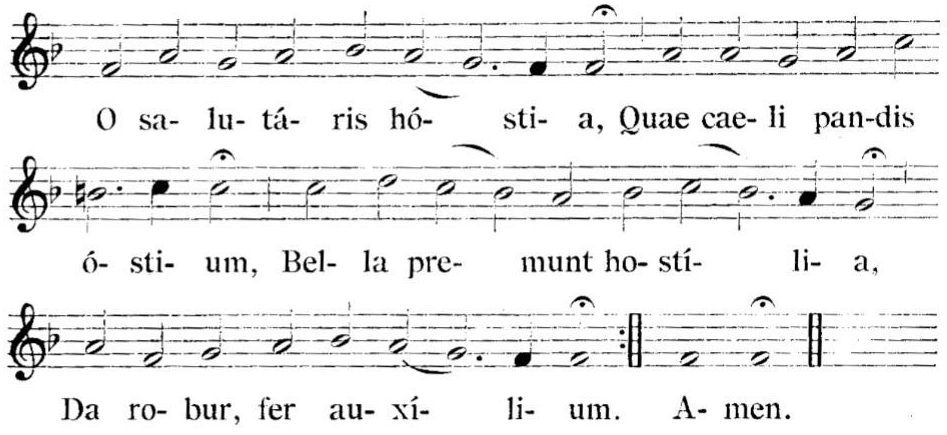
\includegraphics[width=\linewidth]{../ordinaires/o-salutaris.jpg}
  \end{figure}

  \begin{center}
    \begin{footnotesize}
      \textit{
        Ô réconfortante
        Hostie, Qui nous
        ouvres les portes du
        ciel, les armées ennemies
        nous poursuivent,
        Donne-nous la force,
        porte-nous secours.
      }
    \end{footnotesize}
  \end{center}

  \begin{multicols}{2}
    \begin{flushright}
      Uni trinoque Domino\\
      Sit sempiterna gloria :\\
      Qui vitam sine termino,\\
      Nobis donet in patria. Amen.\\
    \end{flushright}
    \columnbreak
    \textit{
      Au Seigneur unique en trois personnes,\\
      La gloire éternelle;\\
      qu'il nous donne en son Royaume\\
      La vie qui n'aura pas de fin. Amen\\
    }
  \end{multicols}

  \begin{center}
    \rule{2cm}{0.4pt}
  \end{center}

  \newpage

  % \begin{center}
  %   \textcolor{red}{\normalsize{Antienne à la Sainte Vierge.}}\\
  % \end{center}
  \begin{center}
    \textcolor{red}{\large{Salve Regína}}\\
    \begin{footnotesize}
      \textit{
      Du Dimanche de Pâques jusqu'au Vendredi après la Pentecôte inclusivement.
      }
    \end{footnotesize}
  \end{center}

  \gresetinitiallines{1}
  \greillumination{\initfamily\fontsize{11mm}{11mm}\selectfont S}
  \gregorioscore{an--salve_regina--solesmes}
  \medskip
  \begin{footnotesize}
    \textit{
      Salut, ô Reine, Mère de Miséricorde, notre vie, notre douceur, et notre espérance, salut. Vers vous nous élevons nos cris, pauvres exilés, malheureux enfants d'Eve. Vers vous nous soupirons, gémissant et pleurant dans cette vallée de larmes. De grâce donc, ô notre Avocate, tournez vers nous vos regards miséricordieux. Et, après cet exil, montrez-nous Jésus, le fruit béni de vos entrailles. Ô clémente, ô miséricordieuse, ô douce Vierge Marie.  
    }
  \end{footnotesize}

  \begin{multicols}{2}
    \parindent=0pt
    \begin{flushright}
      \textcolor{red}{\Vbar.} Ora pro nobis, Sancta Dei Génitrix.\\
      \textcolor{red}{\Rbar.} Ut digni efficiamur promissionibus Christi.\\
    \end{flushright}

    \columnbreak
    
    \textit{\textcolor{red}{\Vbar.} Priez pour nous, Sainte Mère de Dieu. \\
    \textcolor{red}{\Rbar.} Afin que nous soyons rendus dignes des promesses du Christ.}\\
  \end{multicols}

  \begin{multicols}{2}
    \parindent=0pt
    Omnípotens sempitérne Deus, qui gloriósæ Vírginis Matris Maríæ corpus et ánimam, ut dignum Fílii tui habitáculum effici mererétur, Spíritu Sancto cooperánte, præparásti : \textcolor{red}{†} da, ut, cujus commemoratióne lætámur, \textcolor{red}{*} ejus pia intercessióne, ab instántibus malis et a morte perpétua líberémur.\\ Per eúmdem Christum Dóminum nostrum.\\ 
    \textcolor{red}{\Rbar.} Amen.

    \columnbreak

    \textit{Dieu tout-puissant et éternel, qui avez préparé le corps et l’âme de la glorieuse Vierge et Mère Marie afin d’en faire une demeure digne de votre Fils, avec le concours du Saint-Esprit ; faites que, par la prière maternelle de celle dont nous évoquons avec joie la mémoire, nous soyons affranchis du mal présent et de la mort éternelle.\\
    Amen.
    }
  \end{multicols}

  \begin{center}
    \rule{2cm}{0.4pt}
  \end{center}

  \newpage

  \begin{center}
    \textcolor{red}{\large{En l'honneur Du Saint Sacrement}}
  \end{center}

  \gresetinitiallines{1}
  \greillumination{\initfamily\fontsize{11mm}{11mm}\selectfont T}
  \gregorioscore{../ordinaires/hy--tantum_ergo--solesmes}

  \begin{center}
    \begin{footnotesize}
      \begin{enumerate}[label=\textcolor{red}{\emph{\arabic*}}]
        \item \textit{Devant un sacrement si grand, prosternons-nous, adorons ; et que les symboles anciens s'effacent devant le rite nouveau ; que la foi vienne suppléer à la faiblesse de nos sens.}
        \item \textit{Au Père et au Fils louanges et acclamations, gloire honneur et puissance ainsi que bénédictions. A Celui qui de tous deux procède offrons une égale louange.}
      \end{enumerate}
    \end{footnotesize}
  \end{center}

  \medskip

  \begin{multicols}{2}
    \parindent=0pt
    \textcolor{red}{\Vbar.} Panem de caelo praestitisti eis.\\
    \textcolor{red}{\Rbar.} Omne delectamentum in se habentem.\\
    
    \textit{\textcolor{red}{\Vbar.} Tu leur a donné le pain du ciel.\\
    \textcolor{red}{\Rbar.} Toute saveur se trouve en lui.}\\
    
  \end{multicols}

  \bigskip

  \begin{center}
    \textcolor{red}{\large{Oraison}}
  \end{center}

  \begin{multicols}{2}
    \parindent=0pt
    Deus, qui nobis sub sacramento mirabili
    passionis tuæ memoriam reliquisti : \textcolor{red}{~†}
    tribue, quæsumus, ita nos Corporis et
    Sanguinis tui sacra mysteria venerari, \textcolor{red}{~*} ut
    redemptionis tuæ fructum in nobis
    jugiter sentiamus.\\
    Qui vivis et regnas
    cum Deo Patre in unitate Spiritus Sancti,
    Deus, per omnia sæcula sæculorum.
    Amen.
    \columnbreak

    \textit{
      Seigneur Jésus Christ, dans cet admirable
      sacrement tu nous a laissé le mémorial de
      ta passion ; donne-nous de vénérer d’un si
      grand amour le mystère de ton Corps et de
      ton Sang, que nous puissions recueillir
      sans cesse le fruit de ta rédemption. Toi
      qui règnes avec le Père et le Saint Esprit
      pour les siècles des siècles.
      Amen. 
    }
  \end{multicols}

  \begin{center}
    \rule{2cm}{0.4pt}
  \end{center}

  \newpage


  \begin{center}
    \textcolor{red}{\large{Louanges divines}}
  \end{center}


  \begin{normalsize}
    \parindent=0pt
    Dieu soit béni.\\
    Béni soit son Saint Nom.\\
    Béni soit Jésus-Christ, vrai Dieu et vrai homme.\\
    Béni soit le Nom de Jésus.\\
    Béni soit son Sacré Cœur.\\
    Béni soit son précieux Sang.\\
    Béni soit Jésus dans le très Saint Sacrement de l’autel.\\
    Béni soit l’Esprit Saint Consolateur.\\
    Bénie soit l’auguste Mère de Dieu, la très Sainte Vierge Marie.\\
    Bénie soit sa Sainte et Immaculée Conception.\\
    Bénie soit sa glorieuse Assomption.\\
    Béni soit le nom de Marie, Vierge et Mère.\\
    Béni soit Saint Joseph, son très chaste époux.\\
    Béni soit Dieu dans ses anges et dans ses saints.\\
    Seigneur, donnez-nous des prêtres.\\
    Seigneur, donnez-nous de saints prêtres.\\
    Seigneur, donnez-nous beaucoup de saints prêtres.\\
    Seigneur, donnez-nous beaucoup de saintes vocations religieuses.\\
  \end{normalsize}


  % \newpage

  \begin{center}
    \textcolor{red}{\large{Déposition}}\\
    \textit{Psaume 116}
  \end{center}

  \gresetinitiallines{1}
  \greillumination{\initfamily\fontsize{11mm}{11mm}\selectfont L}
  \gregorioscore{../temps_pascal/psaumes/ps--laudate_dominum_omnes_gentes_(psalmus_116)--solesmes}
  \bigskip
  \begin{footnotesize}
    \textit{
      Louez le Seigneur, tous les
      peuples ;
      Fêtez-Le, tous les pays !
      Son Amour envers nous
      S'est montré le plus fort ;
      Eternelle est la Fidélité du
      Seigneur !
      Gloire au Père, au Fils
      Et au Saint-Esprit,
      Comme il était au
      commencement,
      Maintenant et toujours,
      Pour les siècles des siècles,
      amen.
    }
  \end{footnotesize}

\end{document}